\documentclass[dvipdfmx]{standalone}
\usepackage{tikz}
\usetikzlibrary{positioning}

\begin{document}
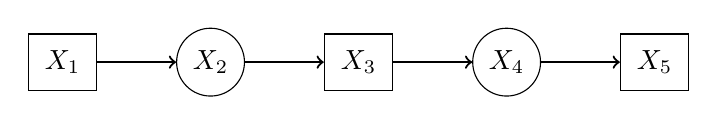
\begin{tikzpicture}[
  nodestyle/.style={
        draw,
        circle
  }
]

    \coordinate (G) at (0cm, 0cm);

    \node[rectangle, draw, inner sep=6] (X_1) {$X_1$};
    \node[nodestyle, right=1cm of X_1] (X_2) {$X_2$};
    \node[rectangle, draw, inner sep=6, right=1cm of X_2] (X_3) {$X_3$};
    \node[nodestyle, right=1cm of X_3] (X_4) {$X_4$};
    \node[rectangle, draw, inner sep=6, right=1cm of X_4] (X_5) {$X_5$};

    \draw[thick, ->] (X_1) -- (X_2);
    \draw[thick, ->] (X_2) -- (X_3);
    \draw[thick, ->] (X_3) -- (X_4);
    \draw[thick, ->] (X_4) -- (X_5);
\end{tikzpicture}
\end{document}
